\documentclass[BIT, graphvis, a4paper]{usydthesis}

\usepackage[final]{pdfpages} 
\usepackage[toc]{appendix}
\usepackage[utf8]{inputenc}
\usepackage{amsfonts}
\usepackage{amsmath}
\usepackage{amssymb}
\usepackage{caption} 
\usepackage{color} 
\usepackage{chngpage}
\usepackage{float}
\usepackage{framed}
\usepackage{fullpage}
\usepackage{titletoc}
\usepackage{graphicx}
\usepackage[a4paper,margin=1.3in,headheight=20pt,footskip=.6in,headsep=.2in]{geometry}
\usepackage{hyperref} 
\usepackage{listings} 
\usepackage{subcaption} 
\usepackage[
	backend=biber,
	natbib=true,
	style=numeric,
	url=true, 
	doi=true,
	eprint=false
]{biblatex}
\usepackage{tabularx} 
\usepackage{tabu} 
\usepackage{tikz} 
\usepackage{url}
\usepackage{wrapfig} 
\usepackage{fancyhdr}
\pagestyle{fancy}

\renewcommand{\sectionmark}[1]{\markright{\thesection.\ #1}}

\fancyhead{} % clear all header fields
\fancyhead[LO,LE]{\leftmark}
\fancyhead[RO,RE]{\thesection}

\fancyfoot{}
\fancyfoot[RO,LE]{\thepage}
\fancyfoot[LO,RE]{Linus Karsai}

\renewcommand{\headrulewidth}{0.4pt}

\addbibresource{bibliography.bib}

% Related work title/citation
\newcommand{\relatedwork}[1]{
	\textit{\citetitle{#1} \textcite{#1}}
}


\usetikzlibrary{arrows}
\usetikzlibrary{shapes,snakes}
\usetikzlibrary{positioning,calc}
\DeclareUnicodeCharacter{00A0}{ }
\newcommand*\rot{\rotatebox{90}}
\makeatletter
\newcommand{\@chapapp}{\relax}%
\makeatother
\graphicspath{ {images/} }
\setlength{\parskip}{\baselineskip}%
\setlength{\parindent}{0pt}%
% graph settings
\definecolor{nodeyellow}{RGB}{255,252,135}
\definecolor{nodeblue}{RGB}{179,255,255}
\tikzset{
	every node/.style={font=\sffamily\scriptsize}
}
\tikzset{
	group/.style={font=\sffamily,fill=nodeblue}
}
\tikzset{
	->,>=stealth',shorten >=1pt,auto,node distance=3cm,
	thick,main node/.style={ellipse,fill=nodeyellow,draw,font=\sffamily\normalsize}
}

% give captions a bit of space.
\captionsetup[sub]{margin=5pt, skip=10pt}

% listings style for prov code
\lstdefinestyle{provn}{
	breaklines=true,
	showstringspaces=false,
	basicstyle=\footnotesize\ttfamily,
}
\lstdefinestyle{basic}{
	breaklines=true,
	showstringspaces=false,
	basicstyle=\footnotesize\ttfamily,
	keywordstyle=\color{black},
	commentstyle=\color{black},
	stringstyle=\color{black},
}


\title{Clustering Provenance}

\begin{document}
\author{Linus Karsai}

\pagenumbering{roman}
\maketitle
\chapter*{Contents}

\startcontents[sections]
\printcontents[sections]{l}{0}{\setcounter{tocdepth}{1}}

\include{abstract} % abstract of thesis

% reset the page numbering and change to arabic numbers
\newpage\setcounter{page}{1}\pagenumbering{arabic}

\chapter{Introduction}

Provenance as a concept has been around for a long time. It originally comes from the Latin word \textit{provenio}, meaning ``to come forth''. It's primary use is in the field of antiques where provenance is used to identify the authenticity and quality of something. For anyone with a backgruond in databases this term may also be fimilair as linking tuples in a query output to the reasons they exist.

In this paper the provenance we refer to is that of \textit{digital provenance}. It is a type of metadata representing the lineage of an object. Naively it can be compared to the information stored in revision history systems like that used in google docs\footnote{Google docs: \url{https://docs.google.com}} or version control
% TODO: git and mercurial links
systems such as git\footnote{GIT\: \url{}} or mercurial. These systems are usually limited to storing revisions as well as authorship. However extends beyond this by making it posible to store and ultimately trace what other things and activities led to a digital object been in its current state.

Provenance has the potential for usefulness in many different fields. The foremost and focus of this paper is the field of personal data management, allowing users to understand how their data is used. Often when a user chooses to share their personal data it is aggregated, anonymised or passed through any number of functions. By exploring provenance users have the ability to understand exactly how much and in what state their personal data is used.

An example to illistrate this point. Alice has a report that describes her current fitness level as well as outlining possible improvements. Viewing the provenance of
% TODO: Fitbit and Withings footnotes
this report shows which sources have been used (e.g. Fit-Bit data to track steps, Withings scale to track weight) and what processes analysed them. In this case it could show that Alice's fitness report was generated using step data from her FitBit data, passed through a summarisation process that summarises 15 minute interval data into daily steps. This shows tracing of lineage backwards in time, it is also possible to trace information forward, possibly in the case of errors in data. Alice remembers that she lent her FitBit to a friend to try for a week, causing errors in her data. Provenance would allow tracing of the errenous information forward to see what other processes and entities it effected and would need to be corrected.

Provenance is also potentially useful in any field where the lineage of an object needs to be stored. This could be extended to digital records of antiques or artwork. This would also be useful in data warehouse systems where information about data transformations as well as origin are stored. There is also research into storing provenance in
% TODO: reference to block chains
block-chains or similar systems to prevent medling of historical data where it to be used in high risk systems such as banks or accounting systems.

Early provenance systems stored provenance information in a variety of different flat
% TODO: prov reference
file formats. Since 2013, the PROV specification has provided a generic model for storing provenance with a number of serialisations (PROV-N, XML, JSON and RDF). PROV identifies provenance elements as three main concepts:

\begin{itemize}
	\item Entities: Physical, digital, conceptual objects
	\item Activities: Elements that cause an entity to come into existence
	\item Agents: Someone or something that can be assigned responsibility for an activity taking place.
\end{itemize}

The industry standard for representing these concepts is on an acyclic graph. An example of this with each of the three main concepts can be see in Figure~\ref{fig:key-concepts}.

\begin{wrapfigure}{r}{0.5\textwidth}
	\centering
	\includegraphics[width=\linewidth]{key-concepts}
	\caption{Key Concepts and relationships from the PROV standard displayed in a labelled acyclic graph.}
	\label{fig:key-concepts}
\end{wrapfigure}

Provenance can be stored in a variety of different granularity's and levels. The main three levels or provenance are system-level, application-level and network level. System level provenance is the lowest level and will often capture operating system activities such as which application ran at what to point to affect a piece of data. Application level provenance is limited to a single application, and will often capture information directly related to the user using that application. Network provenance captures information via network switches and stores lineage originating from multiple machines. These three levels are quire broad and do not cover all use cases but they do give a good point for starting discussion and comparing provenance capture tools. Provenance is also captured at different levels of granularity. Using the example of Alice as above, a system may capture information about her step data at the smallest granularity: how many steps every 15 minutes, or it may store the information at a larger granularity: aggregating step data daily.

As you can see in Figure~\ref{fig:key-concepts} provenance graphs are most often represented as directed acyclic graphs
% TODO: Novel provenance representation citing
although there has been some other novel approaches. The main problem we discuss is  provenance can become incredibly large, particularly in the case of OS level recording as it is usually at a low granularity so a lot of data is been recorded in a small time. Because provenance is inherently historical it is forever growing in size (as of yet there's no standard for going back and ``compressing'' history,) this means even  provenance captured as a high granularity will monotomiously grow and can become a graph with thousands or millions of nodes. This quickly becomes a
% TODO: usability studies chapter cite
usability problem as users can't visually digest such large graphs (results for usability studies in section x show that users are even put off by graphs with as little as 30 nodes).

What we describe in this paper is a process of simplifying graphs by clustering nodes into single composite nodes. A part from simplifying the graph and presenting less objects on screen, this also allows users to control what information is seen by other people or highlight particular concepts as seen in section x.
 % intro to pro etc.

\section{Related work}
\label{sec:related_work}

\subsection{Provenance Overview}
\label{sec:provenance_overview}

As mentioned above, provenance is historically used in the field of antiques as a guide to authenticity of quality. In this thesis we focus on the more modern concept of digital provenance, a metadata that stores the lienage of a file. Only recently defined, below are two papers outlining the requirements and definition of digital provenance.

\relatedwork{Carata2014}
\label{sub:a_primer_on_provenance}

Published in the \textit{Communications of the ACM} magazine, this article gives an in depth introduction to digital provenance. It presents current research in the field from a practical perspective and talks at length about their possible use cases as well as issues obtaining, using and securing provenance.

This paper does an impressive job of laying out the fundamentals of digital provenance, as well as identifying current research efforts and areas of improvement. It also describes the language and terminology used by the provenance community when discussing different features of provenance, such as the concepts of \textit{granularity} and \textit{layering} when collecting provenance.

\relatedwork{Groth2012}
\label{sub:requirements_for_provenance_on_the_web}

This paper from \textit{The International Journal of Digital Curation} synthesizes three main categories that can be used to assess the adequacy of different online provenance systems. It splits these categories into multiple dimensions for finer grained analysis.

The three main categories this paper uses as a base for assessing provenance systems is: content (the data itself and information stored in it), management (different ways of collecting and storing the data) and use (different ways of using the data, visualisation etc.). Each of these categories is then divided into a multitude of related dimensions. For example the \textit{Content} category includes versioning (records of changes written to artefacts over time) and attribution (sources that contributed to making an artefact) as dimensions. The papers support their claims for the requirements of these dimensions by describing them in relation to three scenarios. The scenarios are well picked in order to mirror real world applications.

This paper outlines a range of dimensions that can by used in order to assess an interface. In terms of HCI these can be used as the base for tasks to test on users as well as suggesting features that may be useful in my application. For example, one of the dimensions for \textit{Use} is \textit{Imperfections}, suggesting that I need to take into account that erroneous/imperfect provenance data may exists when creating my interface.

\subsection{Provenance Acquisition}
\label{sec:provenance_acquisition}

Provenance can be acquired in a variety of ways. A common goal in the literature is to collect provenance automatically and transparently in order to reduce cognitive load on users as well as reducing erroneous or false data. The papers below discuss the collection of provenance across two different layers: operating system level and application level, both with their advantages and disadvantages.

\subsubsection{OS level provenance acquisition}
\label{sub:os_level_provenance_acquisition}

OS level provenance acquisition stores the calls between different processes and files. It has the advantage of clearly showing what applications rely on which resources and can be used via a custom kernel to log provenance on a computer without requiring any changes to the users applications.
However because of its intrinsic need to treat processes as ``black boxes'' it can also trigger false positives when graphing lineage. For example a process may invoke the use of multiple libraries however it is arguable as to whether they're all relevant in terms of provenance.

\relatedwork{Muniswamy2006}

Published in 2006, the PASS paper is often cited in related literature as a prime example of OS level provenance collection. This paper discusses the advantages of having provenance information maintained by the storage system as well as presenting a PASS implementation with analysis of its performance costs.

In most implementations provenance is stored in a standalone database systems or flat files. This paper argues that provenance should be maintained by the storage system since it is the storage system that manages existing metadata for files. This allows tighter coupling between data and provenance as well as allowing the transparent collection and management of provenance information. The paper lists a set of requirements for a PASS system as well as their own implementation. They benchmarked their implementation on a 500Mhz Pentium 3 computer with 768MB of RAM. The two primary benchmarks used are small and large file microbenchmarks. In the case of the small file benchmark the overhead associated with creating and writing files was as much as 200\%, however its noted that the absolute numbers are still quite small and that this benchmark in particular is quite challenging to PASS. Results from the large file benchmark where better with a time overhead of no more than \%10-\%20.  It seems more reasonable that real users will only encounter overheads of the latter in daily use. Overall the PASS system provides extra functionality not currently available in other systems with only a moderate overhead. It is also important to note that the systems used for these benchmarks are a lot less powerful that what average users use today.

\subsubsection{Application level provenance acquisition}
\label{sub:application_level_provenance_acquisition}

Application level provenance acquisition has the advantage of creating more relevant relationships between different entities. However it suffers from the overhead required to implement effective capturing and in a lot of cases onus on the user to annotate their actions. Most of the papers below discuss a system that requires developers to somehow modify (usually marginally) their application in order to correctly collect provenance.

\relatedwork{Guo2012}

Authored by Margo Seltzer (one of the top contributors of the field\cite{Macko2012,Seltzer2011,Borkin2013,Muniswamy-Reddy2010,Braun2008},) and Philip J. Guo, this paper presents one of the many ways to collect provenance on a computer. It focuses primarily on research relate provenance and its application in respect to \textit{lab notebooks}.

The application presented in this paper, Burrito, consists of two parts: an extensible platform that automatically captures provenance as well as a set of applications that allow annotations and querying of that data. Stored in a local MongoDB, provenance is captured though GUI window interactions, OS-level capture (like PASS\cite{Muniswamy2006}) and integration with a versioning filesystem. On top of this is a series of plugins that allow provenance to be captured by the following applications: microphone, xpad, Firebox, Chrome, Vim, Bash, Python and the clipboard. Burrito then provides four applications that allow interaction with the provenance data. An activity feed that sits on the users desktop, presenting provenance events chronologically and allowing annotation of events as they happen. A computation context viewer that allows exploration of a files changes and how they impacted output. An activity context viewer that shows what was been read and written at the time of an activity. Finally they also provide a Lab Notebook generator that creates a HTML file summarising the users activities. Over a month this system accumulates approximately 2GB of data and although no benchmarks are reported it is stated to have minimal overhead.

This paper is interesting as it brings provenance to the forefront of the users mind. The goal been that they are constantly annotating and referencing past provenance activities during the length of a project. It also has the added advantage of having images and other program output inline the visualisations.

\relatedwork{Macko2012}

Written in 2012 the authors of this paper Macko and Seltzer are both heavy contributors of the provenance field. Whilst most of the other provenance frameworks mentioned in this review are limited to a particular workflow or language, Macko and Seltzer argue that the real world is a lot more heterogeneous and to accommodate for this they argue the need for a general-purpose provenance library.

This paper presents the Core Provenance Library (CPL) a C++ application that allows the integration of provenance storage into any application. It supports bindings for C, Java and perl as well as a command a line tool for creating shell scripts. The provenance is stored on a database system of your choice through two drivers; these where tested to work for MySQL, PostgreSQl and 4store. The main disadvantage of this framework is that it is the onus of the developers to implement calls to the provenance framework in their application. Multiple features are implemented in order to allow easier integrating such as automatically taking care of persistent storage, cycle detection and resolution, as well as supporting query visualisation through map orbiter~\cite{Seltzer2011}. However developers/project managers need to take into consideration integration when developing an application.

This library provides hope for a standardised way of capturing provenance information. However as mentioned above it is up to developers to correctly integrate it and there's an intrinsic trust that correct and truthful provenance will be recorded. Disappointingly the \href{https://code.google.com/p/core-provenance-library/}{google code repository} hasn't been updated since 2012 and no replacement github repository has been created in light of the shutdown of Google code, suggesting that the project is no longer maintained.

\relatedwork{Allen2010}

This paper describes the ability to compose multiple provenance-unaware services in an ``open world'' system and collect provenance information about their execution. It presents a provenance collection application that sits upon the enterprise service bus (ESB) in order to log provenance information from communicating applications.

This paper advocates for a provenance collection solution that doesn't require system-invasive strategies such as custom kernels or modified applications. It argues that in order to be useful in the ``open world'' provenance capturing tools must fulfil the following tasks, capturing provenance:
\begin{itemize}
  \item across multiple systems with no assumption of control.
  \item from legacy systems
  \item at the level of application interaction, \textit{not} foundational technology stack.
\end{itemize}

In order to evaluate their ESB MULE Capturing Agent (MCA) they tested it upon two different workloads: Loan Borker (a standard MULE test scenario) and CoTLooper (a scenario that uses cursor on target messages). The average time to log provenance within MULE over time decreased as the more provenance nodes where created eventually evening out around $1 \times 10^8ns$. However if message reflection (a method for examining runtime behaviour of applications in the Java VM) was required to gather data from the payload of the message then message capture time can be greatly increased. Whilst these metrics are useful in identifying the overhead of using an ESB to capture provenance information from communicating applications (in this case minimal), itis arguable that the provenance information would suffer from problems similar to OS level capturing systems, creating false positive edges in the graph.

This paper is highly cited in the provenance community. It shows one of the many \textit{layers} of provenance that can be recorded and is one of the few systems that records provenance across multiple machines. 

\subsection{Provenance Storage}
\label{sec:provenance_storage}

Once provenance has been captured by one of the methods mentioned above, it has to be stored somehow. In a lot of early papers the provenance was stored in different proprietary flat file formats. Since then a standard has been created by the W3C, as well as research into how provenance can be stored on the cloud.

\relatedwork{primer2013}

This online document is an initiative by W3C to create a standard as by which to discuss and store digital provenance. This paper is part of a series of documents outlining different aspects of the PROV standard, in particular it is a primer on the fundamental PROV concepts.

This document outlines the three mains concepts illustrated in Figure~\ref{fig:key-concepts}, as well as different serialisations in languages such as XML, JSON and PROV-N. Each of the concepts are briefly described as:
\begin{itemize}
	\item Entities: Physical, digital, conceptual objects
	\item Activities: Elements that cause an entity to come into existence
	\item Agents: Someone or something that can be assigned responsibility for an actity taking place.  
\end{itemize}

\begin{figure}[h]
	\centering
	\includegraphics[width=0.5\linewidth]{key-concepts}
	\caption{Key concepts and relationships from the PROV standard displayed in a labelled acyclic graph.}
	\label{fig:key-concepts}
\end{figure}

I used the standards defined in this paper as the oracle definition for provenance in my designs. My prototype was built so that it can read provenance files in the PROV-N format.

\relatedwork{Muniswamy-Reddy2010}

This paper presents the following problem: although cloud data and provenance both exist, they are not usually used in conjunction because it is difficult to store both in the same location. Traditionally if data is stored in a database, the related provenance information is then stored somewhere else. To mitigate this they present 3 different methods for maintaining data and provenance in current cloud stores.

This paper's contribution is three protocols (using off the shelf software,) each satisfying a different number of properties crucial for provenance systems: provenance data coupling, multi-object casual ordering, data-independent persistence and efficient querying. Each of the systems work with minimal overhead and surprisingly the protocol that fulfils all four of the afore mentioned properties runs as well if not better than the other protocols. The benchmarks used on each of the protocols where varying in their workloads, ranging from CSV backup simulations to workloads representing scientific computation. There is a diverse selection of workloads that simulate scenarios that provenance would most likely be used in.

This creates an avanue of further research. Currently my prototype interface only reads locally stored flat provenance files. In the future it would be useful to expand this to provenance stored on the cloud as well.

\subsection{Provenance Security}
\label{sec:provenance_security}

Once provenance is captured and stored the issue of securing it is paramount. Simple per-attribute access permissions are ineffective for provenance entities because so much information can be gathered from relationships. It is alos worth considernig how to secure the data in such a way that history can't be ``re-written''. The below papers discuss this problem in greater detail.

\relatedwork{Braun2008}

A discussion paper from 2008, Margo, Uri and Avraham focus on the issue of properly securing the access rights of provenance data. It frames the problem and identifies issues requiring further research.

This paper aims to start discussion and highlight the importance of considering provenance security during the implementation and development of an application. It proves that provenance cannot be secured in the same way as traditional data because of its ability to provide information through relations as well as the artefacts themselves, arguing instead that provenance needs its own security model. The paper suggests that there is three main aspects of provenance that needs to be secured, each in their own way: the \textit{node data}, the \textit{relationships} between nodes and the \textit{attributes} related to nodes or relationships. It gives concrete examples of why each of these aspects need to be protected and why regular access control methods aren't satisfactory.

This piece is though provoking in the issues it outlines related to securing provenance. It raises the question of how to present partial graphs caused by users with limited permissions. A problem also worth considering in future work is that of how to present to a moderator which bits of a graph are accesible by who.

\relatedwork{Cheney2011}

A common theme among papers regarding provenance systems is that they agree that provenance is an open and unsolved issue. This paper from the University of Edinburgh outlines a formal model for provenance, formalization of security fundamentals \textit{disclosure} and \textit{obfuscation} and exploration of its implications in various domains.

This paper identifies five main classes of provenance policies: availability, confidentiality, integrity, reverse-engineering and explanation. They go on to describe a high level security framework focusing on the availability (ensuring information about input is available to users) and confidentiality (ensuring that confidential information is never disclosed to a user) of provenance data. This framework is general enough to not be specific to any one system, meaning its rules and obvservations can be applied to any system. The paper provides support to its claims through detailed mathematical proofs. It also provides three instances of how the provenance security framework can be used to create provenance policies.

Unfortunately this paper provides limited benefit to my project because its focus on security is abstract enough to be most useful to researchers designing provenance security systems. However it provides understanding of the security issues involved as well as ideas of how security will be implemented. 

\relatedwork{Hasan2009}

This paper is often referenced because of it work in creating \textit{Sprov}, a secure provenance storage method. 

The author's main contribution from this paper is \textit{Sprov}, a prototype of the secure provenance primitives, implemented as wrapper functions for the standard I/O library in C. They use a chain encryption method in order to accomplish their primary security goal: stopping undetected rewrites of history. In order to evaluate the Sprov library it was run through a number of benchmarks that simulate different deployment settings. They tested two different configurations for chain storage, both recording straight to disk and also storing on RAM with a chrom daemon periodically flushing the chain to disk. Postmart benchmark was used with a dataset containing 20,000 files ranging in size from 8KB to 64KB. Different write loads where tested all the way from 0-100\%. In its worse case scenario of 100\% writes, Sprov had an overhead of 25\% using disk storage and 11\% using RAM. Small and large file microbenchmarks was used to measure the overhead as a percentage of file size. Interestingly smaller files had a larger overhead, this is thought to be attributed to disk caching (similar results have been found by other provenance benchmarks).

This paper shows one of the many ways provenance data can be used and recorded. Its relevancy to my project is in understanding how provenance will be stored and protected as well as issues that arise in a user interface only showing partial data.

\subsection{Provenance Display}
\label{sec:provenance_display}

Lastly we come to the field of thesis. How to display provenance. As mentioned previously, provenance never reduces in size, it is forever expanding and been added to. Issues quickly arrise when trying to present such vast amounts of information. The primary issue been that users can't process such large graphs effectively.

\subsubsection{Visualisation fundamentals}
\label{sub:visualisation_fundamentals}

There's a series of fundamentals that have been tried and tested in the field of visualisation as important rules to follow when developing visualisation tools. Ben Shneiderman discusses fundamental tasks that should be accomplished by visualisation exploration software in order to be effective. A HCI paper then presents how non-technical users view provenance information.

\relatedwork{Shneiderman1996}

Published in 1996 this paper is seen as one of the core papers cited when discussing complex visualisation software. It recommends seven properties that should be implemented by an advanced graphical user interface: overview, zoom, filter, details-on-demand, relate, history and extract. It distils these tasks into what's known as the Visualisation Information Seeking Mantra:

\textit{Overview first, zoom and filter, then details-on-demand}\\
\textit{Overview first, zoom and filter, then details-on-demand}\\
\textit{Overview first, zoom and filter, then details-on-demand}\\
\textit{etc.}

Each of these tasks is explained in great detail with arguments as to why they are necessary. It also provides examples of how different applications have implemented certain tasks, providing an array of examples to research in regard to my project.

I used this paper as a primary starting point when creating my prototype. It was effective as a means of outlining the scope of my application, defining what features where and where not importand.

\relatedwork{Bachour2015}

A Human Centred Technology research project, this paper focuses on collecting feedback from non-expert uses on their understanding of provenance. Through the medium of an online game they explore how well users understand the W3 prov standard\cite{primer2013} and its related artifacts as well as their general opinions and beliefs on provenance data.

The main contributions taken from this paper involved the feedback users gave on the representation of provenance information: one example I found particularly interesting is that a lot of users found the directional arrows confusing. The PROV standard is historical, so directional arrows between nodes are used to represent that something came from something else, however most users found this counter-intuitive and believed that the arrows should have been the other way around to show chronological ordering. The researchers use a game they created based in an Orwellian future in order to explain the concept of provenance. Users were presented with provenance graphs that they had to identify mistakes in. Eight players agreed to hour-long phone interviews and 41 submitted online questionnaires. Although the use of an online game as a usability study is unconventional its merits are well argued in the paper as well as citing other research papers that have used similar methods.

This paper provides some useful feedback from non-technical users as to what issues they perceive when dealing with provenance graphs and allows me to start my interface designs with preliminary user feedback. In conjunction to heuristic feedback the paper also provides some insight into non-expert users opinions on the security/privacy issues of provenance as well as their understanding of its real world applications.

\subsubsection{General Large Graph Visualisation}
\label{sub:large_graph_visualisation}

Effective large graph visualisation is an on open issue in many fields outside of provenance. Both of the visualisation techniques presented below use a clustering mechanism for grouping relevant nodes. 

\relatedwork{Abello2006}

This paper presents an interface for exploring large-scale graphs. The visualisation tool is generic in so far as its made for the exploration of graphs in general. It uses a clustered graph to represent information with the ability to arbitrarily expand and collapse clusters to show sub-graphs.

The paper focuses on creating an interface that can present large-scale graphs to users without been impeded by system performance. This paper goes into quite some depth relating to the algorithms used to cluster nodes as well as methods used to maintain usability with constrained resources (although it is important to note that this was written in 2006 and the issue of constrained resources may not be as relevant today). It also explores issues related to naming clusters: the authors decide on a tag based labelling system that they state is sub-optimal for understanding the contents of a cluster. No formal usability study was undertaken, the authors note that the application was in continuous use by data analysts over the six months preceding publication. It is promising that preliminary feedback was collected in this time (such as users wanting to annotate sections of the graph) and implemented into the application.

This paper's main relation to my research includes the problems tackled when visualising such large graphs. Design decisions related to clustering and pre-processing provided to be useful in creating my interface as well as issues presented in labelling clusters. 

\relatedwork{Schaffer1996}

With this paper been nearly twenty years old its obvious how much younger the provenance research field is in comparison to visualisation. This paper talks about using a novel fish-eye interface in order to show large graphs while allowing users to zoom into particular nodes and not lose context. They also provide usability study results in order to support their claim that fisheye views improve performance compared to traditional variable-zoom interfaces.

This paper sets out to research the problems created by viewing large-scale graphs in a variable zoom interface. The authors create a usability test in order to compare the time taken to complete certain tasks on two interfaces. The first is a variable-zoom interface that allows the user to control the zoom level of the entire graph and pan around to find information. The other is a fisheye interface that clusters nodes and allows expansion of clusters in order to view greater detail. The subjects where asked to act as telephone technicians and had to navigate a network graph in order to identify a broken telephone line as well as rerouting lines in order to `repair' the network. The main metric for identifying interface effectiveness was time (in seconds) taken to complete tasks. Using the fisheye interface users on average completed the task 60 seconds faster than when using the variable-zoom interface. Although not statistically analysed the authors also noted that nearly one third of fish-eye results showed a near optimal route when rerouting, whilst variable-zoom results didn't come close to being optimal.

This paper raises some interesting points about the importance of allowing users to have `peripheral vision' when browsing large complex graphs. There is useful details about how they chose to scale magnified clusters as well as discussion about how to accommodate overlapping clusters. Interestingly they run into similar issues as \cite{Abello2006} when trying to label clusters, except 10 years earlier.  

\subsubsection{Provenance display tools}

There is a diverse range of existing provenance display tools that aim to present provenance to users in an easy to understand way. Whilst most of the applications use a directed acyclic graph to present provenance information, there is also representation through the use of Sankey diagrams and orbital graphs, which depending on what information you wish to portray can sometimes be more effective than DAGs.

\relatedwork{Seltzer2011}

As provenance data becomes more common, the amount of provenance information continues to expand. It is not uncommon for the size of provenance data to greatly outweigh its target file, creating provenance data that has upwards of thousands to millions of nodes. This paper presents a Java application that can be used to visualise large scale provenance graphs through the use of zooming and summation techniques.

This paper's core contribution is a cross-platform Java application, titled ``Map Orbiter'', that can be used to visualise RDF/N3 and OPM formatted provenance data. It simplifies complex graphs by grouping related nodes into \textit{summary nodes} and allows users to view more information about a summary node by \textit{zooming} in. It also supports the filter task, allowing users to pick a subsetof nodes that they would like to view. 

This application is often referenced in other provenance visualisation papers as the primary example of directed acyclic graph visualisation. It focuses on similar issues to my project, but focuses on a Java implementation and reads provenance in the RDF/N3 and OPM format.

\begin{figure}[h]
	\centering
	\includegraphics[width=\linewidth]{maporbiter}
	\caption{A screenshot of Mab Orbiter and its semantic zoom. Left: a high-level view of Linux’s login process and its dependencies. Middle \& Right: the progress of zooming into the bash summary node (in the lower-right corner), representing the login shell and the corresponding user session.}
	\label{fig:maporbiter}
\end{figure}

\relatedwork{Biton2007}

This paper is a demonstration that shows how user views can be used to reduce the amount of information returned by provenance queries. It allows users to select which parts of a provenance graph (referred to in this paper as a \textit{work flow}) they find relevant and have the original graph simplified to only include the parts they picked, as seen in Figure~\ref{fig:zoomuserviews}

Similar to clustering, the ZOOM interface simplifies parts of a provenance graph by collapsing nodes, however instead of creating a cluster object, ZOOM creates a replacement \textit{composite} node. The paper illustrates how it generates provenance information from logs stored on an Oracle warehouse as well as outlining some of the optimisations that can be used in Oracle 10.2 to aid in the generation of immediate provenance. The authors also discuss what properties they believe important when collapsing nodes into composites, what features make a ``good'' user view. These features include preserving the inputs and outputs from relevant nodes and hiding as much detail about irrelevant nodes as possible. In terms of size the examples in this paper are limited to graphs of 19 nodes, although extensions for larger graphs are foreseeable through extensions of the application.

This interface is similar to what I ended up designing and implementing. The primary differences are that my application uses provenance files from the PROV-N standard and that my application is designed for provenance exploration, whilst the ZOOM*UserViews system is aimed at simplifying graphs for use by other people.

\begin{figure}[h]
	\centering
	\includegraphics[width=0.8\linewidth]{zoomuserviews}
	\caption{A Screenshot of the Zoom*UserViews application. On the left is the entire provenance graph with parts selected and on the right is the simplified graph created from the selected parts.}
	\label{fig:zoomuserviews}
\end{figure}


\relatedwork{Hoekstra2014}

This paper presents an application called PRO-O-Vis that uses Sankey Diagrams in order to reflect the flow of information through activities. It discusses the application, reasoning behind representation through Sankey diagrams and a brief evaluation of their application.

This papers main contribution is an online tool that can be used to view provenance information stored in the PROV-O format. Once provenance has been uploaded it generates a viewer that allows exploration of the provenance by selecting an activity to focus on (from a dropdown menu) and presenting its related Sankey diagram. The interface is entirely web based and can be embedded in other websites completely self contained (doesn't require API calls to a server). A brief evaluation of the application has been made using four different sources and issues were found regarding input that had a large number or related activities, this could sometimes cause a delay in generating multiple Sankey diagrams. The paper briefly argues the use of Sankey diagrams over DAG graphs as they more easily allow visualisation of magnitude of flow within a network, comparatively complex DAG graphs can make it hard to view this information.

This application differs from other visualisation tools in the field as it's implemented completely in web tools whilst many of the visualizers run on Java. Because of this it is one of the easiest visualisation tools to install and get running because you mearly have to use a web browser. I used this as inspiration for implementing my prototype as a web application. 

\begin{figure}[h]
	\centering
	\includegraphics[width=0.8\linewidth]{provovis}
\caption{Overview report of a runtime experiment, generated by the Prov-O-Vis system.}
	\label{fig:provovis}
\end{figure}

\relatedwork{Callahan2006}

This is one of the earlier papers mentioning the concept of provenance as we know it today. Published at SIGMOD in 2006, this paper discusses the importance of provenance in generating visualizations. It presents an application called VisTrails that can be used to create visualizations whilst recording provenance during exploration to aid in later scrutiny and replication.

This paper states that existing visualization tools are limited because they do not record the provenance of their outputs. VisTrails improves on the downfalls of existing visualization tools through the use of provenance. This paper was written before any provenance standards~\cite{Macko2012} so the application instead stores all relevant provenance information in an XML formatted file. The application uses provenance in order to record \textit{evolving dataflows}, (where a dataflow is a form of visualization pipeline) allowing the modification of existing dataflows in order to compare and contrast resulting visualisations. Because provenance is captured related to changes to dataflows, it's possible at any point to check the history of a particular dataflow and identify what modifications where made to get to its current state. The VisTrails system was demonstrated through 3 examples although no references are made to any current real life uses of the application.

This paper is interesting as it's one of the earliest papers I've found in my research that identifies the importance of provenance. Its example of using provenance for visualization replication also shows how adaptable provenance can be to different scenarios, particularly its usefulness in exploratory situations. Its an important paper in order to be able to understand how the concept of provenance evolved into its current form.

\begin{figure}[h]
	\centering
	\includegraphics[width=0.9\linewidth]{vistrails}
	\caption{A screenshot of the VisTrails system. On the left you can see the provenance of a figure from a report. On the right is different versions of that figure that have been created.}
	\label{fig:vistrails}
\end{figure}

\relatedwork{Borkin2013}

This paper focuses on the visualisation of provenance information relating to filesystem: the read and writes between processes and files. The authors implement a visualization tool called InProv and both qualitatively and quantitatively compare it's effectiveness to one of the standard provenance visualisation tools Orbiter\cite{Seltzer2011}.

This papers main contributions are: Firstly, qualitative research with domain experts in order to create a set of requirements for a provenance visualiser. Secondly, InProv a provenance visualization tool that uses a radial layout and chronological clustering. Thirdly, a quantitative user study comparing the effectiveness of the two interfaces InProv and Orbiter. The qualitative research was undertaking via semi-structured one hour long interviews. They asked the domain experts to talk about how they used provenance information as well as demonstrating their daily workflows. Using results from the qualitative research they created a set of core tasks they wished to accomplish and used radial visualisation to create the InProv tool. The user study had 27 participants who where asked to accomplish tasks of varying difficulty on both the InProv and Orbiter interfaces. The metrics used to analyse performance where seconds required to complete task as well as percentage of correctly completed tasks. In most cases the difference between time to complete tasks was not significantly different between the two interfaces. However using a new clustering algorithm that clusters nodes based on time of activity (compared to process tree clustering) was shown to have significant improvement on task completion time by as much as 90 seconds.

This paper provides a lot of useful quantitative and qualitative information through its well laid out user studies. Of most interest is the interviews with domain experts. Also the choice of using \textit{time based hierarchical grouping} is of particular interest because of the large impact it had upon improving usability. This paper makes the largest attempt at conducting a usability study and my tasks were influenced by the tasks the use in this paper.

\begin{figure}[h]
	\centering
	\includegraphics[width=0.8\linewidth]{filesystem}
	\caption{A screenshot and mockup of the InProv visualisation interface using radial diagrams.}
	\label{fig:filesystem}
\end{figure}
 % literature review

\section{Contributions}

The related work above shows that a growing amount of research is been conducted in the field of provenance. There's already ways to capture provenance (Section~\ref{sec:provenance_acquisition}) as well as ways to store it once its captured (Section~\ref{sec:provenance_storage}). Research has also been conducted into how to then secure this information so that access can be controlled nor can provenance be altered arbitrarily (Section~\ref{sec:provenance_security}). However there a gap in the research when it comes to creating interfaces that allows users to cluster effectively.

As mentioned in Section~\ref{sec:provenance_display}, there is already some existing applications that can be used to visualise provenance graphs. However most of them lack clustering and in particular clustering from a usability perspective. This leaves the following problem unsolved: \textit{Provenance graphs are too complex for regular users to understand.} 

In the upcoming sections of my thesis I outline and go into detail about my three main contributions to the field:

\begin{itemize}
	\item The design of an interface that enables users to cluster effectively.
	\item The creation of a working prototype that implements the aforementioned design.
	\item An evaluation of the design and prototype: covering learnability, ease of use, efficiency, recovery from errors, user attitude.
\end{itemize}


\chapter{Challenges}

% Clustering introduction, what is it, how does it work?
% Clustering nodes with mouse
% Cluserting with regex
% Useful naming of nodes
% Avoiding false dependencies

Clustering in this paper is the action of taking a set of nodes removing them from the graph and replacing them with a single composite node. An example of this is in
% TODO make figure
Figure~\ref{fig:} where you can see the nodes x, y, z have been clustered to create the composite node named `bananas'. Our focus in this paper is the way users interact with and create composite nodes, we aim to describe a set of features that allows users to effectively and confidently use composite nodes in an effective manner.

From this task of clustering a series usability and technical challenges arise. Mainly the interface for allowing users to cluster, the automatic naming of composite nodes and issues resolving false dependencies caused by clustering. Each of these issues is described in greater detail beolow.

\section{User defined clusters}
\label{sec:user_defined_clusters}

As mentioned above, our focus is to allows users to effectively use clusters. The first method we implemented allows the user to ctrl+click multiple nodes and select the group function from a list of contexual commands (this process is described in
% TODO reference section about interfaces.
greater detail in Chapter~\ref{cha:initial_interface}). This process is however limited to allowing users to group a small amount of nodes and in usability studying users quickly become frustrated even having to group more than three or four nodes via this method.

The challenge is how to create a method for allowing users to cluster a large number of nodes without losing the fine grained control of the above process. We decided to implement a naive search function that runs a regex query on all the properties of a node and hilights any nodes with matching properties.

Future challenges involve allowing users to search for all nodes that match one regex but not another. It would also be useful to only match searches on particular properties of a node, for example a user may only want to match their search on \textit{author} of a node (assuming that property exists\footnote{Breifly discussed in the introduction, the PROV standard allows an arbitraty number of key value properties to be attributed to a node.}). Many users during usability studying requested the ability to cluster all the children of a node, extending from this it would also be useful to allows uers to cluster based on a nodes relationships with other nodes, for example ``Cluster all nodes that match the following regex \texttt{X-tweets|query-X-Time} and are not derived from \texttt{TwitterFeed-time-3}.

Possiblty the biggest challenge in this section would be that of paramaterised clustering. Where a single action by the user would create mutliple clusters. A common clustering we found while studying participants was selecting the entity and the actitvity and creating a composite node of them. In Figure~\ref{fig:search1} they would cluster \texttt{[X-tweets-1, query-X-time-1]}, \texttt{[X-tweets-2, query-X-time-2]} and \texttt{[X-tweets-3, query-X-time-3]} into seperate composite nodes. This would be an ideal use of a paramaterised language that would allow the user to ``group all X-tweets with their corosponding query-X-Time'', however creating a language that is both powerfl and easy to learn and use will be quite a challenge.

A possible future endevour would be automation of clustering. Where the application woudl suggest clusterings based on previous provenance workloads. It may then group together infrequently accessed nodes to make it easier to access infrequently used nodes.

\section{Naming composite nodes}
\label{sec:naming_composite_nodes}

When a composite node is created it must be given a name. In an early version of the ProvOwl system nodes where given short random alhpa-numeric names. We found that this soon made the graph incomprehensible and relied on the user manually 
% TODO Reference interface -> rename section
renaming (described in Section~\ref{sec:}) each node in order for the graph to be usable. 

Ideally an interface would give clusters a name describing the nodes inside of it. However htis requires on domain level knowledge and would even require models of the user and what information is important to them. For example say that the nodes \texttt{sunflower}, \texttt{daphodil} and \texttt{poppies} where to be clustered. Naively it would be useful to name the cluster \textit{plants}, however if the user was a plantologist
% TODO find real name of plantologists
this might be too vague and they would instead prefer to have a node labelled \textit{flowers} or with the root genius of the plants. 

In some fields this problem has been solved by limiting the number of unkowns. If you create a new folder on an iPhone it is automatically named with a label approproate to the applications inside of it. A folder full of photography apps may be labelled \textit{Photography}. However this differs from the problem we are trying to solve in a variety of ways. Firstly the number of possible labels is limited to the categories in the Apple app store, this creates a finite set of possible options. Secondly, when an application is uploaded to the app store the author publishes metadata with it such as the category of the app. Using this metadata makes it much easier to name clustered items. Having the same level of metadata in provenance files could be accomplished by having tags associated with each node. These tags could then be used to effectively name a cluster simply by selecting the most used tag from the group of nodes to be clustered.

Our currently, still simple approach uses the name of the node in the cluster closest to the root with the text ``group'' appended to the end.

\begin{figure}[h]
	\centering
	\includegraphics[width=\linewidth]{naming1}
	\caption{Using the \textit{IR-baseline} example the user has selected four nodes for grouping, essentially those related to \texttt{report-1} and \texttt{report-2}.}
	\label{fig:naming1}
\end{figure}
\begin{figure}[h]
	\centering
	\includegraphics[width=\linewidth]{naming2}
	\caption{When clusterint the four nodes selected in Figure~\ref{fig:naming1} ProvOwl creates a composite node using the name of the node closest to the root (in this case breaking a tie by alphabetical order).}
	\label{fig:naming2}
\end{figure}
\clearpage

\section{False Dependencies}
\label{sec:section_name}

In essense clustering is a simple type of graph rewriting that creates an abstraction of a graph and in turn simplifies deatails. This can cause some anomolies such as false dependencies, circular dependencies and mislabelled relationships. 

A false dependency is when a clustering in the graph has caused a newly implied line of linage that falsly suggests that one enetity had influence upon another. This is in violations of the main assumption that provenance records the factual history of data derivation. The opposite of this, removing a dependency, is not such an issue because it is understood that the ability to observe data trasnformations is limited so therefore all provenaance graphs are expected to be partially incomplete. In Figure~\ref{fig:falsedependencies} you can see a simple example that shows a false dependency caused by joinging nodes \texttt{B1} and \texttt{B2} together. It creates a new line of lineage that falsly implies \texttt{A1} and \texttt{A2} where influenced by \texttt{C1} and \texttt{C2}. Technical consequences of false dependencies also include unnecessary checks and recomputation when revisiting dependent entities to reflect corrected or changed source data. For example if the data in \texttt{C1} was found to be incorrect it would be necessary to follow the lineage up to find what entities need to be recomputed, in the case of Figure~\ref{fig:} (B) this would include both \texttt{A1} and \texttt{A2}.

\begin{figure}[H]
	% TODO fix graph
  \begin{subfigure}[t]{0.5\textwidth}
    \centering
    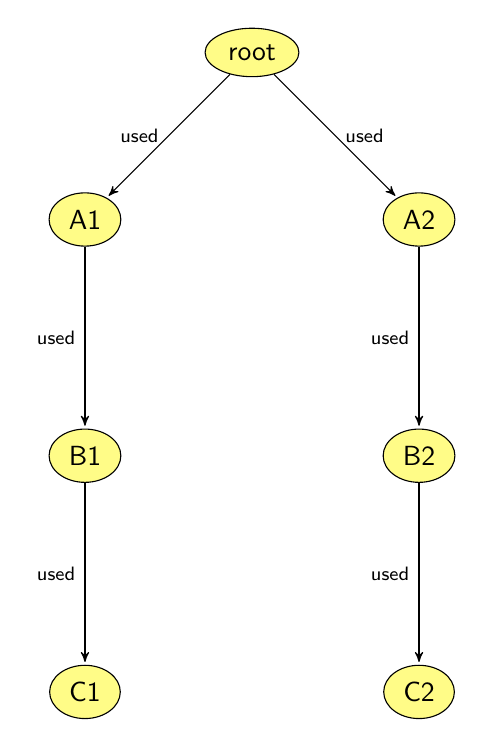
\begin{tikzpicture}
      \node[main node] (root) {root};
	  \node[main node] (A1) [below left of=root] {A1};
      \node[main node] (A2) [below right of=root] {A2};
      \node[main node] (B1) [below of=A1] {B1};
      \node[main node] (B2) [below of=A2] {B2};
      \node[main node] (C1) [below of=B1] {C1};
      \node[main node] (C2) [below of=B2] {C2};
      \path (A1) edge node[left] {used} (B1);
      \path (A2) edge node[left] {used} (B2);
      \path (B1) edge node[left] {used} (C1);
      \path (B2) edge node[left] {used} (C2);
      \path (root) edge node[left] {used} (A1);
      \path (root) edge node[right] {used} (A2);
    \end{tikzpicture}
    \caption{A small example provenance graph that shows two main lines of lineage from the root.}
  \end{subfigure}
  ~
  \begin{subfigure}[t]{0.5\textwidth}
    \centering
    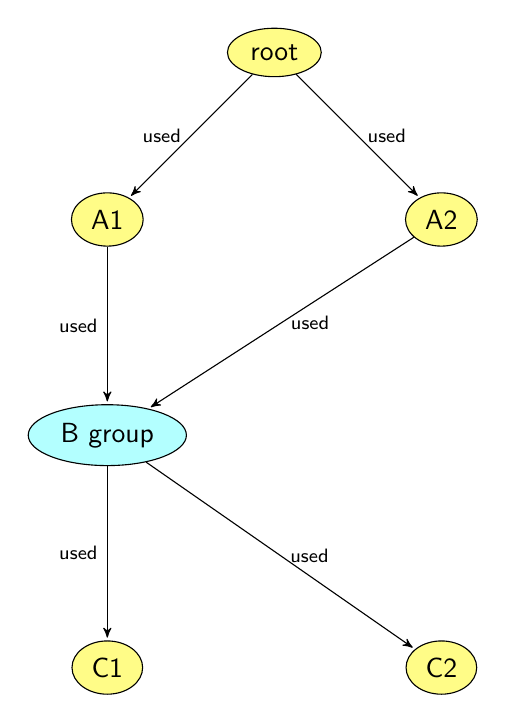
\begin{tikzpicture}
      \node[main node] (root) {root};
      \node[main node] (A1) [below left of=root] {A1};
      \node[main node] (A2) [below right of=root] {A2};
	  \node[main node, group] (CB) [below = 2cm of A1] {B group};
      \node[main node] (C1) [below = 5cm of A1] {C1};
      \node[main node] (C2) [below = 5cm of A2] {C2};
      \path (CB) edge node[left] {used} (C1);
      \path (CB) edge node[right] {used} (C2);
      \path (A1) edge node[left] {used} (CB);
      \path (A2) edge node[right] {used} (CB);
      \path (root) edge node[left] {used} (A1);
      \path (root) edge node[right] {used} (A2);
    \end{tikzpicture}
	\caption{Nodes \texttt{B1} and \texttt{B2} are clustered into the \texttt{B group} composite node.}
  \end{subfigure}
	\label{fig:falsedependencies}
	\caption{When \texttt{B1} and \texttt{B2} are clustered together it creates a false line of lineage that suggests that \texttt{A2} was influenced by \texttt{C2}, this is known as a false dependency.}
\end{figure}

Circular dependencies are another animality that may also occur. This means that the graph is no longer a directed acyclic graph and can cause issues with algorithms that assume the graph is acyclic. It is also in direct violation of the constraints defined in the PROV-CONSTRAINTS W3C document~\cite{}. Figure~\ref{} shows an example of a circular dependency between \texttt{Fitness-Summary group} and \texttt{Summarize}.

The last anomaly that we noticed was that of mislabelled relationships. The labels used to label relationships are specific to the types of nodes the edge is connecting. For example an Entity \textit{was generated by} and Activity, or an Activity was \textit{used} by an Entity. Clustering creates a fourth node type in conjunction with the existing three (Activity, Entity and Agent) and doesn't have any limitation to the labls that can be used on relationships associated with it. This can be confusing to users and can also reveal information about nodes inside a cluster (a used relationship to a cluster node says that there's an entity inside of it). There's also the case of when clustered nodes created multiple relationhips to nodes in common, which relationship label should be picked to represent the relationship? At the moment ProvOwl arbitarily selects one. 

A theoretical formulation of provenance abstraction by clustering has been proposed in~\cite{Missier2014} to discuss this and other problems that occur in clustering, along with simple algorightms for grouping arbitary sets of nodes. In essense the work showed that to avoid false dependencies one must compute a \textit{closure} operation that extends the user-selected nodes with all other nodes that sit on any path amongst these inisial clustering nodes. Combining this work with our user-oriented provenance navigation system can lead to a working correct clustering mechanism. Expanding on the work of this interface to help the user cluster without creating graph anomolies is a challenge we hope to tackle in the future.
 % challenges of clustering

\chapter{Working Prototype}

\section{Functions and Design}

In order to effectively assess the effectiveness of a clustering model we created a prototype interface that could be used to demo the different features when usability testing. We created a web application called ProvOwl that reads provenance from the PROV format and renders a directed acyclic graph that users can explore by panning, zooming and rearranging nodes.

\begin{figure}[h]
\centering
\includegraphics[width=\linewidth]{interface-example}
\caption{A screenshot of ProvOwl rendering the \texttt{fitbit\_score} prov file used in the usability studies.}
\label{fig:interface-example}
\end{figure}

When designing and selecting the features I would implement I used Ben Shneiderman's paper \textit{The eyes have it}~\cite{Shneiderman1996} as a foundation. In this paper he outlines seven visualisation tasks that are a useful starting point for designing advance graphical user interfaces. The tasks (taken directly from Shneiderman's paper) are as follows:

\begin{itemize}
\item Overview: Gain an overview of the entire collection. 
\item Zoom : Zoom in on items of interest 
\item Filter: Filter out uninteresting items. 
\item Details-on-demand: Select an item or group and get details when needed.
\item Relate: View relations hips among items. 
\item History: Keep a history of actions to support undo, replay, and progressive refinement.
\item Extract: Allow extraction of sub-collections and of the query parameters. 
\end{itemize}

Whilst implementing ProvOwl I continually came back to this list of tasks as a grounding point. Below I describe the main features of the interface. 

\subsection{Movement and Rearranging}
\label{sec:movement_and_rearranging}

On first opening a provenance graph, the viewport is positioned to fit an entire graph on screen as seen in Figure~\ref{fig:interface-example}. This acomplishes the \textit{overview} task from above and allows the user to view all the provenance at once. Users can then pan around by clicking and dragging. Zooming is accomplished by pressing ctrl+[+,-] or by using the scroll wheel. In large graphs this allows users to zoom in on areas of interest. 

By default the graph's overall layout is detemined using a JavaScript library called dagre that generates layouts for directed acyclic graphs client side. The main skeleton of the algorithm implemented to acomplish this comes from the paper ``A technique for Drawing Directed Graphs''~\cite{Gansner1993}. In early prototypes other layout options where made available such as circle and breadth-first, but this confused users and where later removed in favor of using dagre exclusively for layout.

\begin{wrapfigure}{r}{0.3\textwidth}
	\centering
	\includegraphics[width=\linewidth]{interface-details-close}
	\caption{A close up of the details panel from Figure~\ref{fig:interface-details}}
	\label{fig:key-concepts}
\end{wrapfigure}

Although initial placement is determined using the dagre algorithm, users can also re-arrange nodes manually by clicking and dragging a node. Note that this causes some issues when users are trying to pan, instead of cliking and dragging the background they accidentally click and move a node instead.

\subsection{Details on demand}
\label{sec:details_on_demand}

When a user selects a single or group of nodes the details panel is shown, as in Figure~\ref{fig:interface-details}. This displays information about the node as well as all its properties. At the bottom of the panel in blue text are contexual hyperlinks that enable functions such as renaming and in the case of multiple selected nodes, grouping. As suggested by the title, this directly immplements the taks of details-on-demand.

\begin{figure}[h]
	\centering
	\includegraphics[width=\linewidth]{interface-details}
	\caption{A screenshot of ProvOwl with the \texttt{IR-baseline} prov file open. A indicated by the red outline, the node \texttt{TwitterFeed-time-1} has been selected and details about it such as name and classification status are shown in the details panel in the top left.}
	\label{fig:interface-details}
\end{figure}

\subsection{Clustering}
\label{sec:clustering}

As mentioned in Section~\ref{sec:user_defined_clusters} I have implemented two ways of clustering nodes, manually and via a search function. In both cases once the user activates the group function, the currently selected nodes are animated to their new position (the node closest to root) and replaced by a composite node, represented by a light blue oval. 

To manually cluster nodes a user first selects multiple nodes at once, by clicking on each whilst holding down \textit{ctrl}. Once multiple nodes have been selected the user cn group them together either with \textit{ctrl+g} or by selecting the group nodes hyperlink from the details panel.

The above method is tedious for more than a handful of nodes so I also implemented the search function. By opening up the search panel the user has access to a search field. The search function takes the value inputted by the user and runs a regex match on each property of each node. If any property of a node matches the regex it is selected (as indicated by a red outline).

In Figure~\ref{fig:search1} you can see an example of this. Open inside the ProvOwl interface is \textit{IR-baseline.prov}, an abstract example that shows the provenance of a report that is created to show analytical information about twitter data from two different users. On the right hand side of the screen is the search panel with the regex text \texttt{X-tweets|query-X-Time}. This query is run on all the nodes and because the pipe (\texttt{|}) characted represents an OR operator in regex hilights all the nodes that are either names \texttt{X-tweets-*} or \texttt{query-X-Time-*}. Once thses nodes are hilighted (as indicated by the red outline) they can be clustered into a composite node as seen in Figure~\ref{fig:search2}.


\begin{figure}[h]
	\centering
	\includegraphics[width=\linewidth]{search1}
	\caption{A screenshot or ProvOwl with the \textit{IR-baseline.prov} file open; an abstract example that shows the provenance of an advice report presenting analytical information about twitter feeds. The search panel has been used to select a subset of the nodes.}
	\label{fig:search1}
\end{figure}
\begin{figure}[h]
	\centering
	\includegraphics[width=\linewidth]{search2}
	\caption{Using the \textit{Group Nodes} button in the search panel, the nodes highlighted in Figure~\ref{fig:search1} have been clustered into a single composite node labelled \texttt{X-tweets-1 group}.}
	\label{fig:search2}
\end{figure}

\clearpage

\subsection{History}
\label{sec:history}

Having the ability to undo and redo actions is one of the above mentioned tasks for designing advance graphical interfaces and I believe one of the most important. It allows users to confidently and safely explore information without fear of causing permanent damage. My interface tracks primarily the movement and clustering of nodes. The undo and redo buttons allow users to step backwards and forwards through these actions. Using the history icon in the top right corner of the interface toggles a history pane (as seen in Figure~\ref{fig:interface-history}) that shows the user what step they are currently at. 

\begin{figure}[h]
	\centering
	\includegraphics[width=0.8\linewidth]{interface-history}
	\caption{In the top right of the interface can be seen the history panel. This indicates what step of history the user is currently at. The user can use the undo and redo commands in the top bar to move backwards and forwards.}
	\label{fig:interface-history}
\end{figure}

\subsection{Sharing}
\label{sec:sharing}

In the top bar of Figure~\ref{fig:interface-history} there is a menu-bar option to export the current graph. This dropdown menu allows the user to either save the entire graph, or just the current viewport, as an image. The option to export just the viewport allows a user to focus on a certain section. This is related to the share task above and allows easy sharing of provenance files with other people for feedback and analysis. In the future I would also like to be able to export the current graph in PROV format with notation for clustered nodes.

\subsection{Click tracker}
\label{sec:click_tracker}

To facilitate with usability testing and by recommendation of Judy Kay I implemented a click tracker into the application. This simply logs clicks that the user makes, capturing time, location and element that the user clicked on. This could then be downloaded via the export command as a CSV file.  You can see below an example of the file generated from exploring the IR-baseline prov file.


\begin{figure}[h]
	\centering
	\lstinputlisting[style=basic]{misc/clickfile.csv}
	\caption{The CSV file generated from a user exploring the IR-baseline provenance file. Each line represent a single click by the user, a small description of the action they completed, what element it effected and the X,Y position of the click (if appropriate).}
	\label{fig:clickfile}
\end{figure}
 % explanation of interface

\chapter{Technical Decisions and Alternatives}

\section{Web Technologies}
\label{sec:web_technologies}

As we saw above, I implemented my prototype as a web application. The criteria for picking an implementation platform was that of accessibility to users and speed of development. Using that criteria I decided to make my prototype a web application as it's only entry barrier to users is that of a modern web browser. Web applications are a field that I have experience with and can quickly develop in. 

There are a few pitfalls to this approach that can be addressed through alternative implementations. Because my application is primarily a prototype for illustrating effective exploration features, the issue of scale is not one that was addressed. If a web application was used for enterprise size provenance files the application may soon run out of resources required to render it.

An alternative to a web application would be to write the prototye in an OS independent language such as Java or Python; this would allow wide accessibility and more fine grained control of machine resources. However if an OS level language was chosen issues could later occur in presenting provenance on mobile devices as there aren't may languages that run on both desktop and mobile devices without heavy modifications. Consequently if an OS dependant languages such as Apple's swift of Microsoft's C\# was used features and code would have to be replicated for the different OS languages (assuming that OS independent accessibility is an important criteria).

The standard technology for data visualisation in a browser is the D3.js\footnote{D3: Data Driven Documents \url{https://d3js.org/}} JavaScript library. However as mentioned earlier, I used Cytoscape.js to implement my interface because it's specifically focused on graph theory and has a lot of inbuilt functions such as rendering and events. If this application was to be re-written using D3, a lot more of the fundemental functions of Cytoscape would have to be written from scratch, however it would allow for more fine-grained control of the appplication, this could particularly be useful when dealing with exceptionally large files.

\section{Client Side Processing}
\label{sec:client_side_processing}

As we saw before, the visualiser loads the file on the client side and renders it locally. When first outlining features of the application I wanted it to be primarily stand alone. This means that even though it can run of a web server, you could just as easily run it locally on your computer with minimal effort because all proccessing and computation is done client side. 

However server side computation may be a useful feature for the future, a server with higher computational power and resources may be able to find and analyze interesting details about the file. The naive approach to accomplishing this would to have the file uploaded to the server, analytics run on the provenance and then results downloaded back to the client. An alternative approach however would to have the client select only the neccessary sectinos required for analysis and send those to the server. The client could then render the provenance locally whilst results where computed and finally render the results onto the already drawn graph. This allows the user to begin exploring the graph immediately as well as minimising the amount of bandwidth used by the application.

\section{Node Clustering}
One of the earliest features we discussed when outlining how to visualise provenance was the ability to cluster and create composite nodes. The feature of allowing multiple nodes to be grouped into a single representative node has two main purposes. Firstly it allows simplification of the graph, this is useful when showing someone a speficit section of the graph as well as easier conceptual understanding when exploring. Secondly it is useful when securing graphs and composite nodes can be used to obviscate information.

Cytoscape.js doesn't have a group feature, so it was required to write one from scratch. The key test for this function is that grouping and ungrouping nodes is undestructive: if a series of nodes are grouped and then ungrouped the resulting graph must be isomorphic to the original.

\begin{figure}[h]
  \centering
  \begin{subfigure}[t]{0.5\textwidth}
    \includegraphics[width=\textwidth]{ungrouped}
    \caption{Graph with no composite nodes}
  \end{subfigure}
  ~
  \begin{subfigure}[t]{0.5\textwidth}
    \includegraphics[width=\textwidth]{grouped}
    \caption{Same graph with a composite node}
  \end{subfigure}
  \caption{An example of a composite node containing the \textit{Tweets}, \textit{X-tweets-1}, \textit{X-tweets-2} and \textit{X-tweets-3} nodes.}
\end{figure}

Nodes removed from Cytoscape.js can be `restored' into their original position, unfortunately any edged associated with the node are permenately destroyed. It is neccessary then to store the edges as a data field in the composite node so that when restoring nodes, edges can also be recreated. 

\begin{figure}[h]
  \centering
  \begin{lstlisting}
 // Create composite node and fields for original edges and nodes.
 Create new CompositeNode 
 CompositeNode.originalEdges = All edges in neighbourhood of selected nodes
 CompositeNode.originalNodes = All nodes that where grouped

 // Create new edges from external nodes to CompositeNode
 for each edge in neighbourhood {
  if (edge != internal to group)  {
    Create new Edge({from: externalNode, to:compositeNode})
  }
 }

 // Remove original nodes
 Remove selected nodes
 \end{lstlisting}
 \caption{Pseudocode: Creaing a composite node}
\end{figure}

However the above code only works in a limited scenario: ungrouping nodes in the oposite order of creation. For example if you created comisite nodes $A$, $B$, $C$ (cronologically and all with neighbouring edges) you would have to ungroup them in the following order: $C$, $B$, $A$. If you where to for example ungroup node $A$ first, when ungrouping $C$ it would try to restore edges to the now non-existent $A$ compsosite node. In order to tackle this I created the group manager class.

The Group Manager class is the primary way of keeping track of nodes that are hidden inside composite nodes. It contains a tree data structure that references all the groups as well as their child nodes/groups. Now when ungrouping nodes this class is called and the parent group of the child node requested, then a new temporary edge is created to the composite node and the original edge stored in a \textit{hanging edges} object until it can be restored. Every time a group is created or destroyed the \textit{hanging edges} object is queried to see if any originl edges can be recreated.

\subsection{Clustering example: Without \textit{Group Manager} or \textit{Hanging Edges}}

Below is an example of issues that occur when trying to ungroup nodes in the incorrect order without the supporting classes \textit{Group Manager} and the hanging edges object. As seen in the final step, all the edges are lost, a less than ideal situation and in failure of the primary test of having an isomorphic graph after grouping and ungrouping nodes.

\begin{figure}[H]

  \begin{subfigure}[t]{0.5\textwidth}
    \centering
    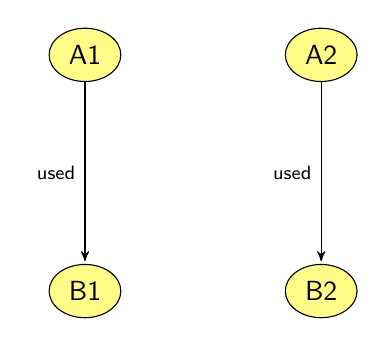
\begin{tikzpicture}
      \node[main node] (A1) {A1};
      \node[main node] (A2) [right of=A1] {A2};
      \node[main node] (B1) [below of=A1] {B1};
      \node[main node] (B2) [below of=A2] {B2};
      \path (A1) edge node[left] {used} (B1);
      \path (A2) edge node[left] {used} (B2);
    \end{tikzpicture}
    \caption{Nodes $A1$ and $B1$ are linked, nodes $A2$ and $B2$ are linked.}
  \end{subfigure}
  ~
  \begin{subfigure}[t]{0.5\textwidth}
    \centering
    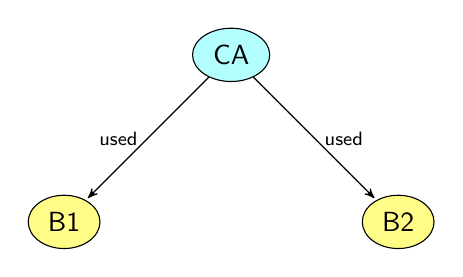
\begin{tikzpicture}
      \node[main node, group] (CA) {CA};
      \node[main node] (B1) [below left of=CA] {B1};
      \node[main node] (B2) [below right of=CA] {B2};
      \path (CA) edge node[left] {used} (B1);
      \path (CA) edge node[right] {used} (B2);
    \end{tikzpicture}
    \caption{Group nodes $A1$ and $A2$ into composite node $CA$. Stored inside the composite node is the original edges from $A1\rightarrow B1$ and $A2\rightarrow B2$.}
  \end{subfigure}
  \begin{subfigure}[t]{0.5\textwidth}
    \centering
    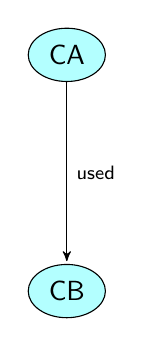
\begin{tikzpicture}
      \node[main node, group] (CA) {CA};
      \node[main node, group] (CB) [below of=CA] {CB};
      \path (CA) edge node[right] {used} (CB);
    \end{tikzpicture}
    \caption{Group nodes $B1$ and $B2$ insto composite nodes $CB$. Stored inside the composite node $CB$ is the edges from $CA\rightarrow B1$ and $CA\rightarrow B2$.}
  \end{subfigure}
  ~
  \begin{subfigure}[t]{0.5\textwidth}
    \centering
    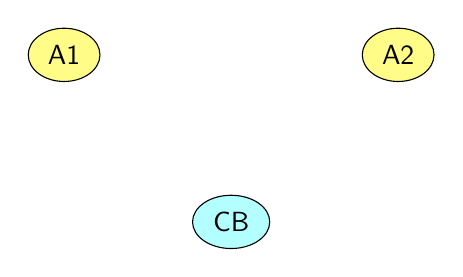
\begin{tikzpicture}
      \node[main node, group] (CB) {CB};
      \node[main node] (A1) [above left of=CB] {A1};
      \node[main node] (A2) [above right of=CB] {A2};
    \end{tikzpicture}
    \caption{Ungroup $CA$. It will try to create adges between $A1\rightarrow B1$ and $A2\rightarrow B2$, because $B1$ and $B2$ are currently in a group, the new edges will fail and not be rendered.}
  \end{subfigure}
  \begin{subfigure}[t]{0.5\textwidth}
    \centering
    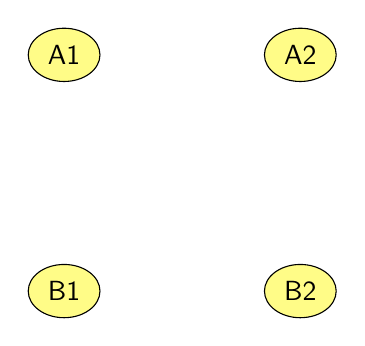
\begin{tikzpicture}
      \node[main node] (A1) {A1};
      \node[main node] (A2) [right of=A1] {A2};
      \node[main node] (B1) [below of=A1] {B1};
      \node[main node] (B2) [below of=A2] {B2};
    \end{tikzpicture}
    \caption{Ungroup $CB$. Edges between $CA\rightarrow B1$ and $CA\rightarrow B2$ will try to be restored but because there's no $CA$ in the graph these will fail.}
  \end{subfigure}
\end{figure}

\subsection{Clustering example: Working isomorphic grouping with helping classes.}
As mentioned previously we want to complete the test of having an isomorphic graph after grouping and ungrouping nodes. To do this we use both a class \textit{GroupManager} and an array \textit{HangingEdges}. The \textit{GroupManager} stores a tree to monitor groups and nodes inside them, it also has some helper functions for adding groups and finding the upmost group of a certain node. The \textit{HangingEdges} array is simply a list of edges that couldn't be restored because one or more of the connected nodes where missing.

In the figure below the left hand side shows the state of the graph, whilst the right hand side shows the \textit{GroupManager} as well as the content of \textit{HangingEdges}.

\begin{figure}[H]

  \begin{subfigure}[t]{0.5\textwidth}
    \centering
    \renewcommand\thesubfigure{A1}
    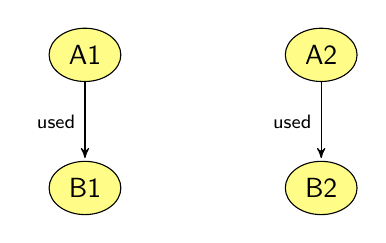
\begin{tikzpicture}
      \node[main node] (A1) {A1};
      \node[main node] (A2) [right of=A1] {A2};
      \node[main node] (B1) [below = 1cm of A1] {B1};
      \node[main node] (B2) [below = 1cm of A2] {B2};
      \path (A1) edge node[left] {used} (B1);
      \path (A2) edge node[left] {used} (B2);
    \end{tikzpicture}
    \caption{Nodes $A1$ and $B1$ are linked, nodes $A2$ and $B2$ are linked.}
  \end{subfigure}
  ~
  \begin{subfigure}[t]{0.5\textwidth}
    \renewcommand\thesubfigure{A2}
    \centering
    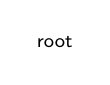
\begin{tikzpicture}
      \node[] (root) {root};
    \end{tikzpicture}
    \caption{The GMTree (Group Manager Tree) is currently empty and Hangingedges = [].}
  \end{subfigure}
  \begin{subfigure}[t]{0.5\textwidth}
    \centering
    \renewcommand\thesubfigure{B1}
    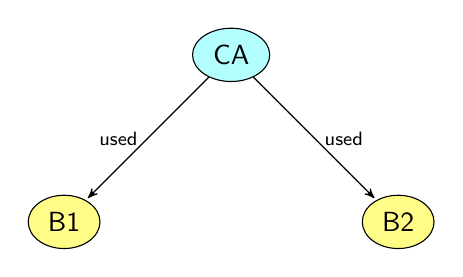
\begin{tikzpicture}
      \node[main node, group] (CA) {CA};
      \node[main node] (B1) [below left of=CA] {B1};
      \node[main node] (B2) [below right of=CA] {B2};
      \path (CA) edge node[left] {used} (B1);
      \path (CA) edge node[right] {used} (B2);
    \end{tikzpicture}
    \caption{Group nodes $A1$ and $A2$ into composite node $CA$. Stored inside the composite node is the original edges from $A1\rightarrow B1$ and $A2\rightarrow B2$.}
  \end{subfigure}
  ~
  \begin{subfigure}[t]{0.5\textwidth}
    \centering
    \renewcommand\thesubfigure{B2}
    \begin{tikzpicture}
      \node[] (root) {root};
      \node[below = 1cm of root] (CA) {CA};
      \node[below right = 1cm of CA] (A1) {A1};
      \node[below left = 1cm of CA] (A2) {A2};
      \path (root) edge (CA);
      \path (CA) edge (A1);
      \path (CA) edge (A2);
    \end{tikzpicture}
    \caption{The GMTree holds information about $CA$, $A1$ and $A2$. Hangingedges = [].}
  \end{subfigure}

  \begin{subfigure}[t]{0.5\textwidth}
    \renewcommand\thesubfigure{C1}
    \centering
    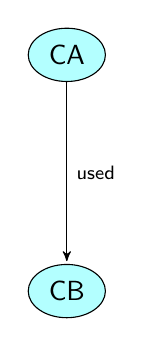
\begin{tikzpicture}
      \node[main node, group] (CA) {CA};
      \node[main node, group] (CB) [below of=CA] {CB};
      \path (CA) edge node[right] {used} (CB);
    \end{tikzpicture}
    \caption{Group nodes $B1$ and $B2$ insto composite nodes $CB$. Stored inside the composite node $CB$ is the edges from $CA\rightarrow B1$ and $CA\rightarrow B2$.}
  \end{subfigure}
  ~
  \begin{subfigure}[t]{0.5\textwidth}
    \centering
    \renewcommand\thesubfigure{C2}
    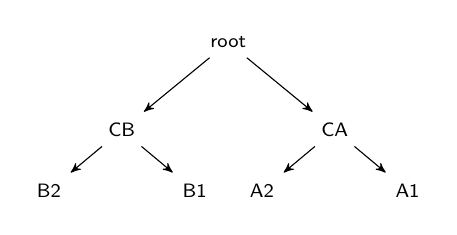
\begin{tikzpicture}
      \node[] (root) {root};
      \node[below right = 1cm of root] (CA) {CA};
      \node[below right = 0.5cm of CA] (A1) {A1};
      \node[below left = 0.5cm of CA] (A2) {A2};

      \node[below left = 1cm of root] (CB) {CB};
      \node[below right = 0.5cm of CB] (B1) {B1};
      \node[below left = 0.5cm of CB] (B2) {B2};
      \path (root) edge (CA);
      \path (CA) edge (A1);
      \path (CA) edge (A2);
      \path (root) edge (CB);
      \path (CB) edge (B1);
      \path (CB) edge (B2);
    \end{tikzpicture}
    \caption{The GMTree holds information about all nodes. Hangingedges = [].}
  \end{subfigure}

  \begin{subfigure}[t]{0.5\textwidth}
    \centering
    \renewcommand\thesubfigure{D1}
    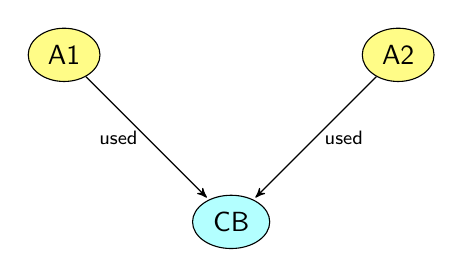
\begin{tikzpicture}
      \node[main node, group] (CB) {CB};
      \node[main node] (A1) [above left of=CB] {A1};
      \node[main node] (A2) [above right of=CB] {A2};
      \path (A1) edge node[left] {used} (CB);
      \path (A2) edge node[right] {used} (CB);
    \end{tikzpicture}
    \caption{CA is ungrouped and removed from the group manager tree. The original edges $A1\rightarrow B1$ and $A2\rightarrow B2$ can't be restored because B1 and B2 are currently hidden inside CB, these edges are stored in the hanging edges object. New edges are created by finding the upmost node using the group manager tree.}
  \end{subfigure}
  ~
  \begin{subfigure}[t]{0.5\textwidth}
    \centering
    \renewcommand\thesubfigure{D2}
    \begin{tikzpicture}
      \node[] (root) {root};
      \node[below = 1cm of root] (CB) {CB};
      \node[below right = 0.5cm of CB] (B1) {B1};
      \node[below left = 0.5cm of CB] (B2) {B2};
      \path (root) edge (CB);
      \path (CB) edge (B1);
      \path (CB) edge (B2);
    \end{tikzpicture}
    \caption{The GMTree holds information about $B$ nodes. $A$ nodes have been remove because they've been ungrouped. Hangingedges = [$A1\rightarrow B1$, $A2\rightarrow B2$].}
  \end{subfigure}

  \begin{subfigure}[t]{0.5\textwidth}
    \centering
    \renewcommand\thesubfigure{E1}
    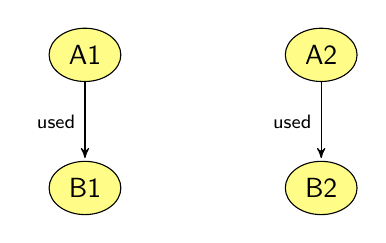
\begin{tikzpicture}
      \node[main node] (A1) {A1};
      \node[main node] (A2) [right of = A1] {A2};
      \node[main node] (B1) [below = 1cm of A1] {B1};
      \node[main node] (B2) [below = 1cm of A2] {B2};
      \path (A1) edge node[left] {used} (B1);
      \path (A2) edge node[left] {used} (B2);
    \end{tikzpicture}
    \caption{CB is ungrouped and removed from the group manager tree. An attempt to restore hanging edges is made and both $A1\rightarrow B1$ and $A2\rightarrow B2$ are restored.}
  \end{subfigure}
  ~
  \begin{subfigure}[t]{0.5\textwidth}
    \centering
    \renewcommand\thesubfigure{E2}
    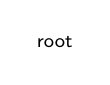
\begin{tikzpicture}
      \node[] (root) {root};
    \end{tikzpicture}
    \caption{The GMTree is empty because there's no groups. Hangingedges = [] because the previously stored edges have been restored.}
  \end{subfigure}
\end{figure}
 % technical implementation decisions

\include{usability-plan} % plan of question coding etc.

\section{Results} % results

\chapter{Conclusions and Discussion} % discussion and future work

Provenance is a type of metadata representing the lineage of a digital object. In the field of personal data management this could be used to help users understand how their personal data is used, an issue that is particulary relevant as we store more and more information about ourselves. The problem is that raw provenance is too difficult to understand and the current industry standard for visualising it (directed acyclic graphs) is still too complex for non technical users (and in a lot of cases technical users). 

To solve this problem I designed two methods for manually clustering nodes, \textit{ctrl+click} and search clustering. Clustering could then be used to simplify provenance graphs in order to hide irrelevant information or focus attention on certain areas of a provenance graph, for example how a single users information was used in a report. I then implemented a working prototype so that a usability study could be conducted on the usability and effectiveness of each clustering technique. Using both a thing aloud study (the gold standard of usability feedback) and a SUS questionnaire (one of the most widely used questionnaires) I conducted a comprehensive usability study on the ProvOwl application. 

The results from the usability study showed that after been prompted to the existence of the clustering function users would use both the \textit{ctrl+click} and search clustering methods in order to simplify graphs. After a small amount of time users were comfortable and confident using the interface to modify graphs to convey meaning, indicating that ProvOwl is a usable interface for clustering graphs.



\section{Future Work}

In the future it would be useful to expand on some of ProvOwl's features as well as implementing some of the other clustering techniques recommended by users in the think aloud study. I would then propose to re-conduct the usability studies and in particular the SUS questionnaire to see if the same divide in results appears.

Future challenges involve allowing users to search for all nodes that match one regex but not another. It would also be useful to only match searches on particular properties of a node, for example a user may only want to match their search on \textit{author} of a node. Many users during usability studying requested the ability to cluster all the children of a node, extending from this it would also be useful to allows user to cluster based on a nodes relationships with other nodes, for example ``Cluster all nodes that match the following regex \texttt{X-tweets|query-X-Time} and are not derived from \texttt{TwitterFeed-time-3}. As mentioned in the think aloud results (\ref{sub:think_alouds}) it would also be useful to have a feature that lets users draw a box over the nodes they want to cluster.

In the future I would also like to expand on the export abilities of the prov owl application to allow exporting in the PROV-N standard. This would allow sharing of provenance graphs with manually created clusters. This would also xxxx expanding the current provenance standard to include syntax for representing nodes that are clustered together.

Lastly, server side computation may be a useful feature for the future, a server with higher computational power and resources may be able to find and analyse interesting details about a file. This could also be used to explore incredibly large provenance files. By having the graph loaded server side and only sections required sent to the client, the computational load on the client could be greatly reduced.


\printbibliography

\newcommand{\multipdf}[4][]{
	\label{sec:#2}
	\includepdf[pages=1,frame=true,width=\linewidth,pagecommand=\section{#2}\label{sec:#3}]{#4}
	\includepdf[pages=2-#1,frame=true,width=\linewidth]{#4}
}

\newcommand{\singlepdf}[3]{
	\includepdf[pages=1,frame=true,width=\linewidth,pagecommand=\section{#1}\label{sec:#2}]{#3}
}

\begin{appendices}
	\stopcontents[sections]
	\chapter*{Appendices}
	\startcontents[appendix]
	\printcontents[appendix]{l}{1}{\setcounter{tocdepth}{2}}
	\renewcommand{\thesection}{\appendixname~\Alph{section}}

	\singlepdf{Provenance Primer}{prov_primer}{pdfs/provenance-primer.pdf}

	\multipdf{Interview Questionnaire}{interview_questionnaire}{pdfs/questionnaire.pdf}

	\multipdf{Participant Information Sheet}{information_sheet}{pdfs/infosheet.pdf}

	\section{PROV File: Alice's Fitness Score}
	\label{sec:prov_file_fitness_score}
	
	\lstinputlisting[style=provn]{misc/fitness-score.provn}

	\clearpage

	\section{PROV File: IR-Baseline}
	\label{sec:prov_file_ir_baseline}
	
	\lstinputlisting[style=provn]{provn/IR-baseline.provn}

\end{appendices}



\end{document}
